
\chapter{Experimental Results}
\label{chap:exp}

In this section. A series of validation experiments for intrinsic calibration, and eye-to-hand calibration are presented. In addition to that, a system validation is carry on for the pipeline pose estimation. In this thesis, two cameras (RealSense D435 and Astra Orbbec) are used.  

In this section the results of the whole system will be shown. A series of validation experiments for the eye-to-hand calibration are presented. 

The performance of the final algorithm will also be evaluated based on the results.

\section{Robot-Camera Calibration}

\subsection{Internal Camera Calibration}
In order to evaluate the accuracy of a single camera calibration, a reprojection error as the only metric is taken in account.  The intrinsic calibration is done with the following packages:


\subsubsection{Reprojection Errors}

Reprojection errors provide a qualitative measure of accuracy. A reprojection error is the distance between a pattern keypoint detected in a calibration image, and a corresponding world point projected into the same image. This should be as close to zero as possible.
Given the intrinsic, distortion, rotation and translation matrices, we first transform the object point to image point using cv2.projectPoints(). Then we calculate the absolute norm between what we got with our transformation and the corner finding algorithm. To find the average error we calculate the arithmetical mean of the errors calculate for all the calibration images.
\begin{itemize}

%lllllllllllllll
\item camera\textunderscore calibration ROS package

\begin{figure}[!h]
\begin{center}
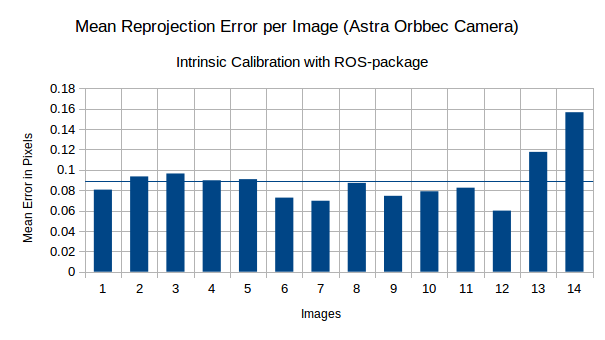
\includegraphics[width=4in]{figures05/ros_int_cal_astra.png}
\caption{ppppppppppp}%\cite{temp2}}
\label{fig:target0}
\end{center}
\end{figure}

\begin{figure}[!h]
\begin{center}
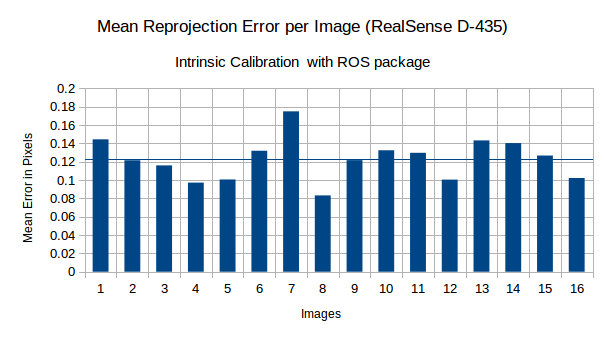
\includegraphics[width=4in]{figures05/ros_int_cal_real.png}
\caption{ppppppppppppp}%\cite{temp2}}
\label{fig:target0}
\end{center}
\end{figure}

%llllllllllllllllllllllllllll
\item OpenCV


\begin{figure}[!h]
\begin{center}
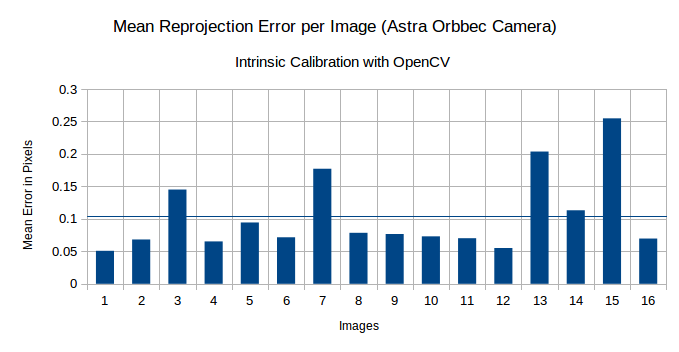
\includegraphics[width=4in]{figures05/opencv_int_cal_astra.png}
\caption{ppppppppppp}%\cite{temp2}}
\label{fig:target0}
\end{center}
\end{figure}

\begin{figure}[!h]
\begin{center}
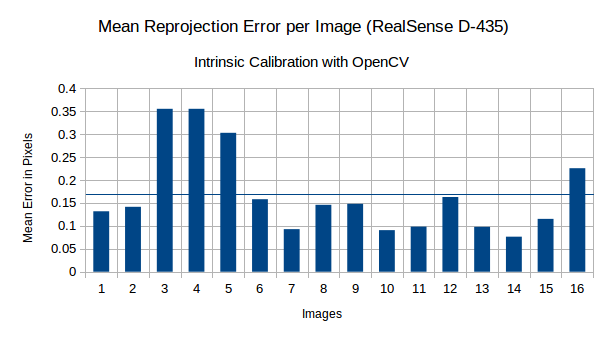
\includegraphics[width=4in]{figures05/opencv_int_cal_real.png}
\caption{ppppppppppppp}%\cite{temp2}}
\label{fig:target0}
\end{center}
\end{figure}


\end{itemize} 



\subsection{External Camera Calibration}


\subsection{Eye-To-Hand Calibration}


\section{Pose Estimation Pipeline}